% !TEX root = ../notes_missingsemester.tex
% Chapter 7: Face the World — Frontend & Nginx
%%%%%%%%%%%%%%%%%%%%%%%%%%%%%%%%%%%%%%%%%%%%%%%%%%%%%%%%%%%%%%%%%%%%%%

\index{Nginx}\index{reverse proxy}\index{frontend}\index{HTTPS}\index{HTTP}\index{TLS}\index{CORS}\index{security headers}\index{HSTS}\index{CSP}\index{JavaScript}\index{HTML}\index{CSS}\index{canvas}
\chapter{Face the World: Frontend \& Nginx}
\printchapterversion{07_frontend_nginx}
\newthought{Browsers do not talk to your app server directly.}

% ==============================================================================================
% BLOCK 1: INTRODUCTION
% ==============================================================================================

\section{The Why}\index{HTTP}\index{Nginx}\index{reverse proxy}

Block~6 left us with a service that classifies and remembers.
\texttt{POST /classify} writes a row, \texttt{GET /results} reads the
twenty most recent predictions, and PostgreSQL keeps the rows around
across restarts.
The contract works for any caller that speaks HyperText Transfer Protocol,
HTTP, and is willing to type an Application Programming Interface, API,
key into a header.
What does not work is a human with a web browser.

\newthought{The only way in today} is a \texttt{curl} one-liner on
port 8000 with a secret header attached.
No \texttt{https://} prefix.
No drawing canvas.
No way to share a link to PixelWise with someone who is not already a
developer.
The service exists, but it has no public face.

\newthought{This block} closes that gap.
We put Nginx\index{Nginx} in front of \texttt{uvicorn}\index{uvicorn},
serve a small static frontend out of \texttt{/opt/pixelwise/frontend/},
move the public surface from plain HTTP on port 8000 to HyperText Transfer
Protocol Secure, HTTPS, on port 443, and route browser traffic through the
same \texttt{POST /classify} and \texttt{GET /results} handlers we wired up
in Block~6.
Figure~\ref{fig:reverse_proxy_flow} shows the request path end to end.

\begin{figure}
\centering
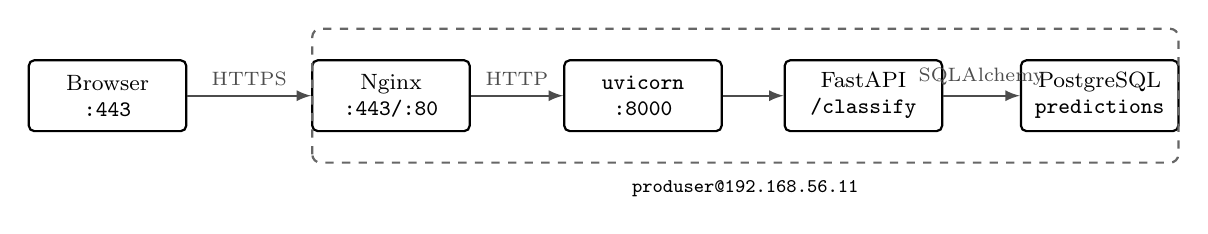
\begin{tikzpicture}[
    every node/.style={font=\footnotesize, align=center},
    box/.style={rectangle, draw=black, thick, rounded corners=2pt, minimum width=2.0cm, minimum height=0.9cm, inner sep=4pt},
    arr/.style={-latex, thick, black!70}
]
\node[box] (br)  at (-1.2, 0) {Browser\\\texttt{:443}};
\node[box] (ng)  at (2.4, 0)  {Nginx\\\texttt{:443/:80}};
\node[box] (uv)  at (5.6, 0)  {\texttt{uvicorn}\\\texttt{:8000}};
\node[box] (fa)  at (8.4, 0)  {FastAPI\\\texttt{/classify}};
\node[box] (pg)  at (11.4, 0) {PostgreSQL\\\texttt{predictions}};
\draw[arr] (br.east) -- node[above]{\scriptsize HTTPS} (ng.west);
\draw[arr] (ng.east) -- node[above]{\scriptsize HTTP} (uv.west);
\draw[arr] (uv.east) -- (fa.west);
\draw[arr] (fa.east) -- node[above]{\scriptsize SQLAlchemy} (pg.west);
\draw[black!60, thick, dashed, rounded corners=3pt]
    (1.4, -0.85) rectangle (12.4, 0.85);
\node[font=\scriptsize, anchor=north] at (6.9, -0.95)
    {\texttt{produser@192.168.56.11}};
\end{tikzpicture}
\caption{\rule{0pt}{1.4cm}\\
Request flow after Block~7. The browser opens a Transport Layer Security,
TLS, connection to Nginx on port 443. Nginx terminates the TLS, serves the
static frontend from disk, and forwards every request prefixed with
\texttt{/api/} to \texttt{uvicorn} on localhost port 8000. FastAPI executes
the same handlers from Block~6 and SQLAlchemy reads and writes rows in
PostgreSQL. The dashed box marks the boundary of the \texttt{prod} VM:
Everything inside runs on one host, but only Nginx is exposed to the
network.}
\label{fig:reverse_proxy_flow}
\end{figure}

\newthought{A reverse proxy} is a server that accepts a request on behalf
of another server, makes the upstream call itself, and returns the
response to the client.
The client only ever talks to the proxy.
The upstream service, in our case \texttt{uvicorn} on port 8000, never
sees the public network directly.
We can change the upstream, restart it, scale it, or swap it for another
process, and the public URL does not move.
That decoupling is the headline of this block.

\newthought{Why not run \texttt{uvicorn} on port 443 directly?}
On Linux, ports below 1024 are privileged: A process needs root, or
explicit capabilities granted by root, to bind to them.
We do not want our application code running as root.
We do not want our application process owning the TLS private key.
We do not want the same process that classifies digits to be responsible
for negotiating cipher suites and parsing HTTP headers from the open
network.
A small, dedicated proxy at the edge handles the privileged port and the
TLS handshake; the application keeps running unprivileged on a high
port and trusts the proxy to filter the traffic that reaches it.

\subsection{Hands On Experience}

\newthought{Consider this scenario:} A classmate watches you demo
PixelWise and asks for the link so they can try it from their laptop.
You open a terminal, scroll back through your shell history, and copy
the \texttt{curl} one-liner that pipes a hand-crafted Java\-Script Object
Notation, JSON, body to \texttt{http://192.168.56.11:8000/classify} with
an \texttt{X-API-Key} header attached.
The classmate stares at the line, blinks, and asks whether there is just
a URL.
There is not.
Not yet.

\newthought{The product is invisible} until you give it a front door.
A URL someone can type into a browser, a page that renders without an
API key tutorial, and a lock icon next to the address are the difference
between a service that exists and a service that other people can use.
This block builds that front door.

\newthought{This seventh block}\index{PixelWise} introduces the public
surface for PixelWise.
By the end you will have
\begin{itemize}
    \item installed and configured Nginx as a reverse proxy on \texttt{prod},
    \item served a static HTML and JavaScript drawing frontend from \texttt{/opt/pixelwise/frontend/},
    \item generated a self-signed TLS certificate and wired it into the Nginx server block,
    \item redirected port 80 traffic to port 443 so every visitor lands on HTTPS,
    \item configured Cross-Origin Resource Sharing, CORS, middleware on FastAPI as defense in depth,
    \item added the security headers \texttt{Strict-Transport-Security}, \texttt{X-Content-Type-Options}, \texttt{X-Frame-Options}, and \texttt{Content-Security-Policy} to every response,
    \item and reached the live application in a browser at \texttt{https://192.168.56.11}.
\end{itemize}

\marginnote{\newthought{The proxy-to-service jump.}\index{reverse proxy}
A service speaks HTTP on a high port to anyone who can reach it.
A proxied service speaks HTTP on a high port only to its proxy and lets
the proxy be the public face.
The work in this block is what turns the first into the second; the
classifier itself does not change.}

% ==============================================================================================
\newpage
\section{Optional Exercise: Catch Up to \texttt{v0.5}}\index{exercises}\index{Git!tag}\index{recovery}

\marginnote{\newthought{Tag map.}\index{Git!tag}
\texttt{v0.5} marks the end of Block~6, \texttt{v0.6} will mark the end
of this block.
Browse the full set at
\url{https://github.com/schutera/pixelwise/tags}.}

\newthought{Catching up via tag.}\index{Git!tag}\index{recovery}
This catch-up extends the one in Block~6. If you have not done that
one, do it first: It lands you at \texttt{v0.4}, the end-of-Block~5
state. The exercise here picks up from there and rewinds to
\texttt{v0.5}, the end-of-Block~6 state, with PostgreSQL provisioned
on both VMs, the \texttt{pixelwise} role and database created, the
SQLAlchemy \texttt{Prediction} model wired into the FastAPI handlers,
and \texttt{POST /classify} writing rows that \texttt{GET /results}
reads back. The optional Alembic exercise from Block~6 sits past the
\texttt{v0.5} tag, so this catch-up does not assume \texttt{alembic/}
or the \texttt{client\_ip} column exists.

\newthought{Both VMs again.} Block~6 ended with the service persisting
predictions on both \texttt{dev} and \texttt{prod}, so this catch-up
brings both machines up to \texttt{v0.5}. The Git-tracked changes
since \texttt{v0.4} include \texttt{app/models.py} with the
\texttt{Prediction} class, \texttt{init\_db.py} for one-shot schema
creation, an updated \texttt{app/main.py} where \texttt{POST /classify}
writes a row and \texttt{GET /results} returns the twenty newest, an
extended \texttt{requirements.txt} adding \texttt{sqlalchemy} and
\texttt{psycopg2-binary}, a \texttt{setup-server.sh} with
\texttt{postgresql} added to the \texttt{apt install} line and an
idempotent provisioning stanza for the \texttt{pixelwise} role and
database, and a refreshed \texttt{.env.example} carrying
\texttt{DB\_PASSWORD} and \texttt{DATABASE\_URL}. The local
\texttt{.env} on each VM needs \texttt{DB\_PASSWORD} written by hand,
and \texttt{DATABASE\_URL} interpolates it at source time so the secret
lives in one place.

\newthought{Run the catch-up on \texttt{dev}.}
Rewind the repository to \texttt{v0.5}, edit \texttt{.env} to set
\texttt{DB\_PASSWORD} alongside the \texttt{SECRET\_API\_KEY} from
Block~5, reinstall pinned dependencies, run \texttt{setup-server.sh}
to install PostgreSQL and provision the role and database, then run
\texttt{python init\_db.py} once to create the \texttt{predictions}
table. The exact commands are in the margin.

\marginnote{\newthought{Sequence on \texttt{dev}.}\\[0.4em]
\texttt{cd \textasciitilde/pixelwise}\\
\texttt{git fetch origin -{}-tags}\\
\texttt{git reset -{}-hard v0.5}\\
\texttt{cp .env.example .env}\\
\texttt{nano .env}\\
\texttt{source .venv/bin/activate}\\
\texttt{pip install -r requirements.txt}\\
\texttt{bash setup-server.sh}\\
\texttt{python init\_db.py}\\[0.3em]
Edit \texttt{.env} to set \texttt{DB\_PASSWORD} to any string of your
choosing and keep the \texttt{SECRET\_API\_KEY} from Block~5.
\texttt{DATABASE\_URL} comes from \texttt{.env.example} and
interpolates \texttt{DB\_PASSWORD} at source time, no manual edit
needed. If you already have a working \texttt{.env}, skip the
\texttt{cp} and just append \texttt{DB\_PASSWORD} in place. If
\texttt{.venv/} is missing, run \texttt{python3 -m venv .venv} before
the \texttt{source} step.}

\newthought{Run the catch-up on \texttt{prod}.}
Same sequence on \texttt{prod}, where \texttt{setup-server.sh}
installs PostgreSQL, provisions the role and database, and restarts
the systemd-supervised \texttt{uvicorn} as it did in Block~5. After
\texttt{python init\_db.py} creates the table, verify the wiring is
sound by hitting \texttt{GET /results} from \texttt{dev}; an empty
list is the right answer.

\marginnote{\newthought{Sequence on \texttt{prod}.}\\[0.4em]
\texttt{ssh produser@192.168.56.11}\\
\texttt{cd /opt/pixelwise}\\
\texttt{git fetch origin -{}-tags}\\
\texttt{git reset -{}-hard v0.5}\\
\texttt{cp .env.example .env}\\
\texttt{nano .env}\\
\texttt{source .venv/bin/activate}\\
\texttt{pip install -r requirements.txt}\\
\texttt{bash setup-server.sh}\\
\texttt{python init\_db.py}\\[0.3em]
Then from \texttt{dev}:\\
\texttt{curl -s http://192.168.56.11:8000/results}\\
should return \texttt{\{"results":[]\}}.}

\marginnote{\newthought{Already have a fork?}\index{Git!fork}
If your own fork carries the \texttt{v0.5} tag, swap \texttt{origin} on
\texttt{dev} with
\texttt{git remote set-url origin git@github.com:<you>/pixelwise.git}
so push and pull continue to target your account.
The HTTPS clone on \texttt{prod} stays read-only.}

\newthought{You are now} at the state where Block~6 ended, with both
machines aligned, ready to start Block~7.

% ==============================================================================================
% BLOCK 2: CONCEPTS AND PRACTICE
% ==============================================================================================

\newpage
\section{Reverse Proxies and Nginx}\index{Nginx}\index{reverse proxy}

\newthought{A reverse proxy sits at the edge.}\index{reverse proxy}
The client opens a connection to the proxy, the proxy opens a connection
to the upstream, and the response flows back along the same path.
The client never knows whether one upstream answered or ten, whether the
upstream lives on the same host or in another data centre, or whether the
proxy rewrote a header on the way through.
The proxy is a contract: A stable public URL with hidden internals.

\marginnote{\newthought{Forward versus reverse.}\index{proxy}
A forward proxy sits in front of the client and reaches out to many
servers on the client's behalf, the way a corporate web filter does.
A reverse proxy sits in front of the server and serves many clients on
the server's behalf.
Same word, opposite direction.}

\newthought{Nginx} is the reverse proxy this course uses.\marginnote{Nginx\index{Nginx}:
\url{https://nginx.org/}\\
Nginx documentation: \url{https://nginx.org/en/docs/}}
It is fast, well documented, and the most common piece of software you
will find sitting in front of Python and Node services in production.
The configuration is a tree of nested blocks: A top-level \texttt{http}
context, \texttt{server} blocks inside it, and \texttt{location} blocks
inside each \texttt{server}.
Each \texttt{server} block declares a listen port and a hostname; each
\texttt{location} declares how to handle requests whose paths match a
pattern.
That is the whole model.

\newthought{Three roles in one process.}
In the PixelWise stack Nginx wears three hats at once.
As a static file server, it ships HTML, CSS, and JavaScript from
\texttt{/opt/pixelwise/frontend/} to the browser as fast as the kernel
can read them.
As a reverse proxy, it forwards every request whose path begins with
\texttt{/api/} to \texttt{uvicorn} on \texttt{localhost:8000}.
As a TLS terminator, it holds the certificate and the private key, so
the public connection is encrypted while the internal connection to
\texttt{uvicorn} stays plain HTTP.

\marginnote{\newthought{Why a high port?}\index{ports}
On Linux, ports below 1024 are privileged; binding requires either root
or a capability granted by root.
\texttt{uvicorn} runs as the unprivileged \texttt{produser}, so it
listens on port 8000 where no special permission is needed.
Nginx is started by \texttt{systemd} as root, binds 80 and 443, then
drops its worker processes to an unprivileged user.
The split keeps application code far away from \texttt{uid 0}.}

\newthought{The directives we will use} are a small subset:
\texttt{listen} names the port, \texttt{server\_name} names the host the
block answers to, \texttt{root} points at the static file directory,
\texttt{location} matches a path prefix, \texttt{proxy\_pass} hands the
request to an upstream URL, \texttt{proxy\_set\_header} copies request
metadata to the upstream so the application sees the real client
address, \texttt{return 301} issues a permanent redirect,
\texttt{ssl\_certificate} and \texttt{ssl\_certificate\_key} point at
the certificate and private key on disk, and \texttt{add\_header}
attaches a response header on the way out.
Every line in the configuration we are about to write is one of these.

\marginnote{\newthought{\texttt{proxy\_pass} is the headline.}\index{reverse proxy}
A single line, \texttt{proxy\_pass http://localhost:8000/}, is what makes
Nginx a reverse proxy.
Without the trailing slash on the proxied URL, Nginx forwards the full
incoming path; with it, the matched location prefix gets stripped before
forwarding.
\texttt{/api/classify} therefore reaches \texttt{uvicorn} as
\texttt{/classify}, which is exactly the route FastAPI registered.}

\newthought{\texttt{nginx -t}} is the cheapest debugging tool in the
chapter.
It parses the configuration without applying it, prints \texttt{syntax
is ok} when the file is well formed, and points at the line and column
of the first problem when it is not.
Run it before every \texttt{systemctl reload nginx} and the daemon will
never refuse to start because of a missing semicolon or a typo in a
directive name.

% ==============================================================================================
\newpage
\section{Exercise: Install Nginx and the First Proxy Pass}\index{exercises}\index{Nginx}

\newthought{Install Nginx on \texttt{prod}.}
On a fresh \texttt{prod} VM, install the package and confirm the daemon
is up and listening on port 80:

\begin{verbatim}
ssh produser@192.168.56.11
sudo apt update
sudo apt install -y nginx
systemctl status nginx --no-pager
\end{verbatim}

\marginnote{\newthought{The default site.}\index{Nginx}
A fresh install ships an Nginx \texttt{Welcome} page from
\texttt{/etc/nginx/sites-enabled/default}.
We will leave it in place until our own site is ready, then disable it
in one step so there is no confusion about which configuration is
serving requests.}

The first three lines should report \texttt{Active: active (running)}.
Visit \texttt{http://192.168.56.11} from your host browser; the default
Nginx welcome page proves the daemon is reachable on port 80 of the VM
over the host-only network.

\newthought{Author the site configuration on \texttt{dev}.}
The Nginx configuration is part of how the application runs, so it
belongs next to the code, the systemd unit, and the setup script.
Open the new file at \texttt{deploy/pixelwise.nginx} in the repository
on \texttt{dev}:

\begin{verbatim}
cd ~/pixelwise
nano deploy/pixelwise.nginx
\end{verbatim}

The file below is the first cut, plain HTTP on port 80, the frontend
served from disk, every request under \texttt{/api/} forwarded to
\texttt{uvicorn}:

\begin{verbatim}
# deploy/pixelwise.nginx
server {
    listen 80;
    server_name 192.168.56.11;

    # Serve the static frontend
    location / {
        root /opt/pixelwise/frontend;
        index index.html;
        try_files $uri $uri/ =404;
    }

    # Forward API calls to uvicorn
    location /api/ {
        proxy_pass http://127.0.0.1:8000/;
        proxy_set_header Host $host;
        proxy_set_header X-Real-IP $remote_addr;
        proxy_set_header X-Forwarded-For $proxy_add_x_forwarded_for;
        proxy_set_header X-Forwarded-Proto $scheme;
    }
}
\end{verbatim}

\marginnote{\newthought{Trailing slash matters.}\index{proxy\_pass}
\texttt{proxy\_pass http://127.0.0.1:8000/} strips the matched
\texttt{/api/} prefix before forwarding.
Without the trailing slash, \texttt{/api/classify} would reach
\texttt{uvicorn} as \texttt{/api/classify} and FastAPI would answer
\texttt{404} because the route is registered as \texttt{/classify}.
One character, opposite outcomes.}

\marginnote{\newthought{\texttt{try\_files} is the static fallback.}\index{try\_files}
For a single-page frontend like ours, the directive tries the requested
path, then a directory listing, then returns \texttt{404}.
A more elaborate frontend with client-side routing would fall back to
\texttt{index.html} instead so deep links survive a reload.
Our app has one page, so the \texttt{404} fallback is correct.}

\newthought{Commit on \texttt{dev}, pull on \texttt{prod}.}
The configuration belongs in the repository so a fresh VM can pick it up
from a clean clone instead of from somebody's terminal history:

\begin{verbatim}
cd ~/pixelwise
git add deploy/pixelwise.nginx
git commit -m "Add Nginx reverse proxy config"
git push
\end{verbatim}

Then on \texttt{prod}, pull the file into place:

\begin{verbatim}
ssh produser@192.168.56.11
cd /opt/pixelwise
git pull
\end{verbatim}

\newthought{Install the site on \texttt{prod}.}
Nginx looks for active sites under \texttt{/etc/nginx/sites-enabled/}.
The conventional pattern is to keep the real files under
\texttt{sites-available/} and symlink the active ones into
\texttt{sites-enabled/}, so disabling a site is one \texttt{rm} away:

\begin{verbatim}
sudo cp deploy/pixelwise.nginx \
    /etc/nginx/sites-available/pixelwise
sudo ln -sf /etc/nginx/sites-available/pixelwise \
    /etc/nginx/sites-enabled/pixelwise
sudo rm -f /etc/nginx/sites-enabled/default
sudo nginx -t
sudo systemctl reload nginx
\end{verbatim}

\marginnote{\newthought{Reload, not restart.}\index{Nginx}
\texttt{systemctl reload nginx} tells the master process to re-read the
configuration and gracefully replace its workers without dropping any
in-flight connection.
\texttt{restart} would kill the master and start it again, briefly
closing the listening sockets.
Reload is the default for configuration changes; restart is for the rare
case where reload is not enough.}

\newthought{Create the frontend directory.}
The \texttt{location /} block points at \texttt{/opt/pixelwise/frontend/}
as the document root.
That directory does not exist yet on \texttt{prod}, and the next
exercise will fill it.
For now, drop a placeholder so the proxy pass has something to serve
when the path is \texttt{/}:

\begin{verbatim}
sudo mkdir -p /opt/pixelwise/frontend
echo "PixelWise frontend stub" | \
    sudo tee /opt/pixelwise/frontend/index.html
\end{verbatim}

\newthought{Did the proxy take?}\index{verification}
From \texttt{dev}, hit the proxied API and the static path back to back:

\begin{verbatim}
curl -s http://192.168.56.11/
curl -s http://192.168.56.11/api/health
\end{verbatim}

\marginnote{\newthought{Did it take on \texttt{prod}?}\index{verification}
\texttt{curl -s http://192.168.56.11/} should print the placeholder text.
\texttt{curl -s http://192.168.56.11/api/health} should print
\texttt{\{"status":"ok","model\_version":"v1"\}}.
The first answer came from Nginx reading a file on disk; the second
travelled from Nginx to \texttt{uvicorn} on port 8000 and back.
The browser sees one origin, \texttt{http://192.168.56.11}, even though
two very different processes produced the two responses.}

The first line should print \texttt{PixelWise frontend stub}.
The second should print the same JSON \texttt{uvicorn} would have given
you on port 8000, except now Nginx is the one that took the request.
Two different programs answered two paths, and from the outside they
look like one service on one port.

% ==============================================================================================
\newpage
\section{The Static Frontend}\index{frontend}\index{HTML}\index{JavaScript}\index{canvas}

\newthought{HTML for structure, CSS for layout, JavaScript for
behaviour.}\index{HTML}\index{CSS}\index{JavaScript}
Those are the three pieces a browser needs to render an interactive
page, and those are the three files PixelWise ships.
HyperText Markup Language, HTML, describes the document tree.
Cascading Style Sheets, CSS, describe how the tree looks.
JavaScript, JS, describes what happens when the user clicks, draws, or
types.
The browser is the runtime; the network is the transport; the server is
just a file system that happens to speak HTTP.

\marginnote{\newthought{Why no framework?}\index{frontend}
React, Vue, and Svelte solve problems that show up at scale: Component
reuse across dozens of views, state management across complex
interactions, routing across many pages.
PixelWise has one page, one canvas, one results panel.
A framework would add a Node.js toolchain, a bundler, a learning curve
orthogonal to this course, and an extra layer hiding the bytes that
actually travel between browser and server.
Vanilla JS keeps the HTTP layer visible.\\
Mozilla Developer Network, MDN: \url{https://developer.mozilla.org/}}

\newthought{The page is a single canvas, one button, and a list.}
The drawing area is a \texttt{<canvas>} element sized at 280 by 280
pixels on screen, which the JavaScript downscales to 28 by 28 before
sending it to the API.
A \texttt{Classify} button extracts the pixel array and posts it.
A results panel renders the predicted digit, the confidence, and a
scrolling history pulled from \texttt{GET /api/results}.
That is the whole user surface.

\newthought{The \texttt{fetch} call} is the bridge between the browser
and the backend.\index{fetch}
\texttt{fetch} is the browser's modern HTTP client, a Promise-based
function that takes a URL and an options object and returns a response
the JavaScript can read as JSON, text, or bytes.
A \texttt{POST} to \texttt{/api/classify} carries the pixel array in
the body and the API key in a header, and waits for the JSON answer:

\begin{verbatim}
async function classifyDrawing() {
    const pixels = getPixelsFromCanvas();  // 28 by 28 array
    const response = await fetch("/api/classify", {
        method: "POST",
        headers: {
            "Content-Type": "application/json",
            "X-API-Key": API_KEY
        },
        body: JSON.stringify({ pixels: pixels })
    });
    const result = await response.json();
    displayResult(result);
}
\end{verbatim}

\marginnote{\newthought{Same-origin by design.}\index{same-origin}
The page is served from \texttt{https://192.168.56.11/} and posts to
\texttt{/api/classify} on the same host.
The browser treats both as the same origin because the scheme, host, and
port all match.
That is why no CORS preflight fires here, and why CORS will only matter
later as defense in depth.}

\marginnote{\newthought{Open by design.}\index{API!authentication}\index{X-API-Key}
The \texttt{X-API-Key} header sits on \texttt{POST /api/classify}
because that endpoint is gated.
\texttt{GET /api/results} and \texttt{GET /api/health} carry no header
because they are unprotected: The browser renders the results panel and
probes the service without juggling a secret in client-side JavaScript.
Anyone who can reach the host can read both right now.
That is acceptable for the demo data here; in a real product
\texttt{/api/results} would sit behind a session cookie or a short-lived
token from a proper login flow.}

\newthought{The relative path is the headline.}\index{URL design}
\texttt{fetch("/api/classify", \dots)} does not name a hostname or a
port.
It resolves against the URL the page itself was loaded from, which is
\texttt{https://192.168.56.11/}.
That single design choice means the same JavaScript runs unchanged in
the classroom on \texttt{https://192.168.56.11} and in production on
\texttt{https://pixelwise.example.com}.
The frontend has zero knowledge of where the backend lives because the
backend lives wherever the frontend was served from.

% ==============================================================================================
\newpage
\section{Exercise: Build and Deploy the Frontend}\index{exercises}\index{frontend}

\newthought{Create the frontend directory on \texttt{dev}.}
The three files live in the repository under \texttt{frontend/} so they
travel with the code, get reviewed in pull requests, and reach
\texttt{prod} through the same Git path as the Python:

\begin{verbatim}
cd ~/pixelwise
mkdir -p frontend
nano frontend/index.html
\end{verbatim}

The HTML is small.
One canvas, one button, one results panel, one stylesheet link, and one
script tag at the bottom so the document tree is built before the
JavaScript looks for elements in it:

\begin{verbatim}
<!doctype html>
<html lang="en">
<head>
    <meta charset="utf-8">
    <meta name="viewport"
        content="width=device-width, initial-scale=1">
    <title>PixelWise</title>
    <link rel="stylesheet" href="style.css">
</head>
<body>
    <h1>PixelWise</h1>
    <p>Draw a digit, then click Classify.</p>
    <canvas id="pad" width="280" height="280"></canvas>
    <div class="controls">
        <button id="classify">Classify</button>
        <button id="clear">Clear</button>
    </div>
    <div id="result"></div>
    <h2>Recent predictions</h2>
    <ul id="history"></ul>
    <script src="app.js"></script>
</body>
</html>
\end{verbatim}

\marginnote{\newthought{Why a 280-pixel canvas?}\index{canvas}
The model expects 28 by 28 grayscale pixels.
Drawing at that size on a modern display would feel like trying to write
on a postage stamp.
The page draws at ten times the model resolution and the JavaScript
downsamples before sending, so the user gets a comfortable pad and the
model gets the input shape it was trained on.}

\newthought{Author the stylesheet} next to the HTML.
The styling is minimal: A centred column, a visible canvas border, a
button row, and a results panel.
The point is readability, not visual design:

\begin{verbatim}
nano frontend/style.css
\end{verbatim}

\begin{verbatim}
body {
    font-family: system-ui, sans-serif;
    max-width: 480px;
    margin: 2rem auto;
    padding: 0 1rem;
}
canvas {
    border: 1px solid #333;
    background: #fff;
    touch-action: none;
    display: block;
}
.controls { margin: 0.5rem 0 1rem 0; }
button {
    padding: 0.5rem 1rem;
    margin-right: 0.5rem;
    font-size: 1rem;
}
#result {
    font-size: 1.25rem;
    min-height: 1.5rem;
    margin-bottom: 1rem;
}
#history li { font-family: monospace; }
\end{verbatim}

\newthought{Author the script.}\index{JavaScript}
\texttt{frontend/app.js} wires the canvas to the mouse, builds the pixel
array, posts it, renders the prediction, and refreshes the history list.
Open the file:

\begin{verbatim}
nano frontend/app.js
\end{verbatim}

\begin{verbatim}
// frontend/app.js
const API_KEY = "REPLACE_ME";  // overwritten on deploy

const pad = document.getElementById("pad");
const ctx = pad.getContext("2d");
let drawing = false;

ctx.fillStyle = "#fff";
ctx.fillRect(0, 0, pad.width, pad.height);
ctx.lineWidth = 18; ctx.lineCap = "round";

pad.onmousedown = e => {
    drawing = true; ctx.beginPath();
    ctx.moveTo(e.offsetX, e.offsetY);
};
pad.onmousemove = e => {
    if (!drawing) return;
    ctx.lineTo(e.offsetX, e.offsetY); ctx.stroke();
};
pad.onmouseup = pad.onmouseleave = () => { drawing = false; };

function getPixels() {
    // Downsample 280x280 -> 28x28, invert so ink is high.
    const tmp = document.createElement("canvas");
    tmp.width = 28; tmp.height = 28;
    tmp.getContext("2d").drawImage(pad, 0, 0, 28, 28);
    const data = tmp.getContext("2d")
        .getImageData(0, 0, 28, 28).data;
    const pixels = [];
    for (let y = 0; y < 28; y++) {
        const row = [];
        for (let x = 0; x < 28; x++)
            row.push(255 - data[(y * 28 + x) * 4]);
        pixels.push(row);
    }
    return pixels;
}

async function classify() {
    const r = await fetch("/api/classify", {
        method: "POST",
        headers: {
            "Content-Type": "application/json",
            "X-API-Key": API_KEY
        },
        body: JSON.stringify({ pixels: getPixels() })
    });
    const out = document.getElementById("result");
    if (!r.ok) { out.textContent = "Error " + r.status; return; }
    const d = await r.json();
    out.textContent = `Prediction: ${d.prediction} ` +
        `(${(d.confidence * 100).toFixed(1)}%)`;
    refresh();
}

async function refresh() {
    const r = await fetch("/api/results");
    if (!r.ok) return;
    const ul = document.getElementById("history");
    ul.innerHTML = "";
    for (const row of (await r.json()).results) {
        const li = document.createElement("li");
        li.textContent = `${row.prediction}  ` +
            `${row.confidence.toFixed(2)}  ${row.created_at}`;
        ul.appendChild(li);
    }
}

document.getElementById("classify").onclick = classify;
document.getElementById("clear").onclick = () => {
    ctx.fillStyle = "#fff";
    ctx.fillRect(0, 0, pad.width, pad.height);
    document.getElementById("result").textContent = "";
};
refresh();
\end{verbatim}

\marginnote{\newthought{Why invert the channel?}\index{MNIST}
The MNIST training set stores digits as light strokes on a dark
background, with zero meaning empty and high values meaning ink.
The canvas draws black on white, the opposite convention.
\texttt{255 - data[i]} flips the polarity so the model sees the input
distribution it was trained on.
Skip the inversion and the classifier will report \texttt{8} for a blank
canvas because the white background looks like a dense glyph.}

\marginnote{\newthought{The API key in client code.}\index{API!authentication}
\texttt{const API\_KEY} sits in plaintext JavaScript that any visitor
can view, so it is not a real secret.
That is fine for the classroom: The host-only network limits who can
reach the page in the first place.
In a real deployment, the gate moves to a session cookie issued after a
login, and the API key never appears in browser-visible code.
We keep the header here so the contract from Block~5 stays intact.}

\newthought{Commit, push, pull.}
On \texttt{dev}, stage the three files and push:

\begin{verbatim}
cd ~/pixelwise
git add frontend/
git commit -m "Add static drawing frontend"
git push
\end{verbatim}

On \texttt{prod}, pull and copy the directory into the document root.
The repository is a Git clone under \texttt{/opt/pixelwise/}; the
\texttt{location /} block in our Nginx config looks at
\texttt{/opt/pixelwise/frontend/}, so a copy is enough:

\begin{verbatim}
ssh produser@192.168.56.11
cd /opt/pixelwise
git pull
sudo cp -r frontend/* /opt/pixelwise/frontend/
\end{verbatim}

\marginnote{\newthought{Wipe and start fresh.}\index{recovery}
If the frontend stub from the earlier exercise is still in place, the
\texttt{cp} overwrites \texttt{index.html} but leaves it lying around.
A clean reset is\\[0.3em]
\texttt{sudo rm -rf /opt/pixelwise/frontend/*}\\
\texttt{sudo cp -r frontend/* /opt/pixelwise/frontend/}\\[0.3em]
followed by a reload of Nginx so any opened file handles refresh.}

\newthought{Edit the API key in place.}\index{X-API-Key}
The script ships with \texttt{const API\_KEY = "REPLACE\_ME"}; the value
that actually works lives in \texttt{/opt/pixelwise/.env} as
\texttt{SECRET\_API\_KEY}.
On \texttt{prod}, replace the placeholder so the deployed script carries
a real key.
A small \texttt{sed} command keeps it auditable:

\begin{verbatim}
KEY=$(grep ^SECRET_API_KEY /opt/pixelwise/.env \
    | cut -d= -f2)
sudo sed -i \
    "s/REPLACE_ME/$KEY/" \
    /opt/pixelwise/frontend/app.js
\end{verbatim}

The same pattern will move into \texttt{setup-server.sh} a few exercises
from now, so a fresh provision picks up the right key without any
manual editing.

\newthought{Did the frontend take?}\index{verification}
Open \texttt{http://192.168.56.11/} in your host browser.
You should see the heading, the canvas, two buttons, and an empty
recent-predictions list.
Draw a clear digit, click \texttt{Classify}, and read the result line.
The history list should grow by one entry, and a refresh of the page
should leave the entry in place because it now lives in PostgreSQL.

\marginnote{\newthought{Did it take?}\index{verification}
If the page loads but \texttt{Classify} produces \texttt{Error 401},
the API key in \texttt{app.js} does not match the one in \texttt{.env}.
If the page loads but \texttt{Classify} produces \texttt{Error 404},
the \texttt{proxy\_pass} trailing slash got lost in a save.
If the page does not load at all, run \texttt{sudo nginx -t} on
\texttt{prod}: A syntax error in the config block keeps the daemon from
applying the new configuration.}

% ==============================================================================================
\newpage
\section{TLS and HTTPS}\index{TLS}\index{HTTPS}

\newthought{Plain HTTP travels in the clear.}\index{HTTP}
A request to \texttt{http://192.168.56.11/api/classify} carries the
pixel array, the path, and every header, including \texttt{X-API-Key},
as readable bytes on the wire.
On a host-only network with two VMs that is mostly a theoretical risk.
On a public network it is a credential leak waiting for the first packet
capture.
The fix is Transport Layer Security, TLS, which encrypts everything
between browser and server with a key the two parties agree on at
handshake time.

\newthought{HTTPS is HTTP over TLS.}\index{HTTPS}
Same protocol, same methods, same headers, same status codes.
A TLS handshake opens before the first HTTP byte, the rest of the
connection is encrypted, and the browser shows a lock icon to tell the
user the channel is private.
Nginx holds the certificate and the private key, so the TLS layer lives
in one place at the edge of the system.

\marginnote{\newthought{TLS in three sentences.}\index{TLS}
The server presents a certificate that binds a hostname to a public key.
The browser checks the certificate against a trust store of known
authorities.
If the certificate validates, the two sides agree on a session key with
public-key cryptography, then encrypt the rest of the conversation
symmetrically.\\
TLS overview: \url{https://datatracker.ietf.org/doc/html/rfc8446}}

\newthought{A self-signed certificate} is a certificate the server
signed itself.\index{certificate}
It carries the same public-key cryptography as one from a public
authority, encrypts the channel just as well, and shows up in browser
warnings because the browser does not recognise the signer.
For the classroom that warning is part of the lesson: It tells you, in
visible language, that the chain of trust between your browser and a
random IP address is exactly as long as you would expect, which is
zero.
A real deployment would replace the certificate with one from
Let's Encrypt or a commercial certificate authority, the rest of the
configuration stays the same.

\newthought{The mechanics are a one-liner.}\index{openssl}
\texttt{openssl req -x509} generates a private key and a self-signed
certificate together, writes the key under \texttt{/etc/ssl/private/}
where only root can read it, and writes the certificate under
\texttt{/etc/ssl/certs/} where every process can.
The \texttt{-nodes} flag asks \texttt{openssl} not to encrypt the
private key file, so Nginx can read it on boot without a passphrase.
The \texttt{-days 365} flag sets a year-long validity window, plenty
for a classroom artefact and absurdly long for a production secret.
The exercise below has the full command.

\marginnote{\newthought{Why redirect HTTP to HTTPS?}\index{redirect}
A user who types \texttt{192.168.56.11} into the address bar lands on
plain HTTP, and the browser will happily speak HTTP to a server that
also speaks HTTPS.
A permanent redirect on port 80 to the same path on port 443 promotes
every such request to the encrypted channel, so credentials never travel
in the clear by accident.
The redirect goes in its own \texttt{server} block, listening on port
80, with a single \texttt{return 301} directive.}

% ==============================================================================================
\newpage
\section{Exercise: Enable HTTPS}\index{exercises}\index{HTTPS}\index{TLS}

\newthought{Generate the self-signed certificate on \texttt{prod}.}
The command writes two files and prompts for the certificate fields.
Press Enter through the prompts except for Common Name, where you type
the IP address the browser will use to reach the site:

\begin{verbatim}
ssh produser@192.168.56.11
sudo openssl req -x509 -nodes -days 365 \
    -newkey rsa:2048 \
    -keyout /etc/ssl/private/pixelwise.key \
    -out /etc/ssl/certs/pixelwise.crt \
    -subj "/CN=192.168.56.11"
\end{verbatim}

\marginnote{\newthought{The \texttt{-subj} shortcut.}\index{openssl}
\texttt{-subj "/CN=192.168.56.11"} skips the interactive prompts and
sets Common Name in one line, which is what
\texttt{setup-server.sh} will want when it provisions a fresh VM.
For a hand-typed one-off, omit the flag and answer the prompts; the only
field that matters for browser matching is Common Name.}

The \texttt{ls -l /etc/ssl/private/pixelwise.key} that follows should
report \texttt{-rw-r-{}-r-{}-} owned by \texttt{root}: The private key is
on disk and unreadable by ordinary users.

\newthought{Update the Nginx site on \texttt{dev}.}
The HTTP-only server block from the earlier exercise becomes two
blocks: One that listens on port 80 and redirects to HTTPS, and one
that listens on port 443 with TLS and carries the full configuration.
Replace the contents of \texttt{deploy/pixelwise.nginx} with:

\begin{verbatim}
# deploy/pixelwise.nginx
server {
    listen 80;
    server_name 192.168.56.11;
    return 301 https://$host$request_uri;
}

server {
    listen 443 ssl;
    server_name 192.168.56.11;

    ssl_certificate     /etc/ssl/certs/pixelwise.crt;
    ssl_certificate_key /etc/ssl/private/pixelwise.key;
    ssl_protocols       TLSv1.2 TLSv1.3;

    location / {
        root /opt/pixelwise/frontend;
        index index.html;
        try_files $uri $uri/ =404;
    }

    location /api/ {
        proxy_pass http://127.0.0.1:8000/;
        proxy_set_header Host $host;
        proxy_set_header X-Real-IP $remote_addr;
        proxy_set_header X-Forwarded-For $proxy_add_x_forwarded_for;
        proxy_set_header X-Forwarded-Proto $scheme;
    }
}
\end{verbatim}

\marginnote{\newthought{Two blocks, one site.}\index{Nginx}
The first block exists only to redirect.
The second block does the actual work.
A request to \texttt{http://192.168.56.11/api/results} hits the first
block, gets a \texttt{301} pointing at
\texttt{https://192.168.56.11/api/results}, the browser follows it, and
the second block answers from inside the encrypted channel.}

\newthought{Commit and deploy.}
On \texttt{dev}, push the updated configuration:

\begin{verbatim}
cd ~/pixelwise
git add deploy/pixelwise.nginx
git commit -m "Enable HTTPS and redirect port 80 to 443"
git push
\end{verbatim}

On \texttt{prod}, pull and reinstall the site.
The certificate is already on disk from the \texttt{openssl} command, so
Nginx only needs the updated configuration:

\begin{verbatim}
ssh produser@192.168.56.11
cd /opt/pixelwise
git pull
sudo cp deploy/pixelwise.nginx \
    /etc/nginx/sites-available/pixelwise
sudo nginx -t
sudo systemctl reload nginx
\end{verbatim}

\newthought{Open it in the browser.}
Visit \texttt{https://192.168.56.11/}.
The browser shows a warning page about an untrusted certificate, which
is the expected outcome for a self-signed certificate: The browser does
its job, refuses to silently trust an unknown signer, and asks the user
to acknowledge the risk.
Click through, in Chrome and Edge that means \texttt{Advanced} then
\texttt{Proceed to 192.168.56.11 (unsafe)}, and the site loads.
The page itself is identical to what you saw on plain HTTP, but the URL
now starts with \texttt{https://}.

\marginnote{\newthought{The warning is the lesson.}\index{security}
A self-signed certificate encrypts the channel just as well as a real
one; what it cannot do is prove who the server is.
The browser warning is the visible sign of that gap.
Replace the certificate with one from Let's Encrypt and the warning
disappears, the encryption does not change at all.}

\newthought{Did it take?}\index{verification}
Confirm both ports answer correctly from \texttt{dev}:

\begin{verbatim}
curl -I http://192.168.56.11/
curl -I -k https://192.168.56.11/
\end{verbatim}

The first response should start with \texttt{HTTP/1.1 301 Moved
Permanently} and carry a \texttt{Location:} header pointing at the
HTTPS URL.
The second should start with \texttt{HTTP/1.1 200 OK} and serve
\texttt{index.html}.
The \texttt{-k} flag on the second call tells \texttt{curl} to accept
the self-signed certificate without complaint, the equivalent of clicking
through the browser warning.

% ==============================================================================================
\newpage
\section{CORS: Cross-Origin Resource Sharing}\index{CORS}

\newthought{Same-origin is the default browser policy.}\index{same-origin}
A page loaded from \texttt{https://192.168.56.11/} is allowed to make
HTTP requests back to \texttt{https://192.168.56.11/} without any extra
ceremony, because the scheme, host, and port all match.
A page loaded from \texttt{https://other.example/} is not allowed to
read responses from \texttt{https://192.168.56.11/} unless the second
server explicitly opts in.
That opt-in is Cross-Origin Resource Sharing, CORS, and it is the most
common deployment puzzle a frontend developer hits in their first year
of shipping web applications.

\newthought{Why does CORS exist at all?}\index{security}
Because the browser holds the user's cookies, authentication tokens, and
session state for every site they have ever visited, and it will gladly
attach those credentials to any request it sends.
Without same-origin protection, a malicious page could trigger requests
to your bank in the background and read the responses.
CORS is the negotiation that lets a server declare which other origins
may read its responses, which methods they may use, and which headers
they may send.

\marginnote{\newthought{The preflight.}\index{CORS!preflight}
For requests with custom headers or non-trivial methods, the browser
sends an \texttt{OPTIONS} request first, asking the server whether the
real request is allowed.
The response carries \texttt{Access-Control-Allow-Origin},
\texttt{Access-Control-Allow-Methods}, and
\texttt{Access-Control-Allow-Headers} listing what is permitted.
Only then does the browser send the real request.
A failed preflight prints the famous \texttt{has been blocked by CORS
policy} message in the developer console.\\
CORS reference: \url{https://developer.mozilla.org/en-US/docs/Web/HTTP/CORS}}

\newthought{Our frontend is same-origin.}
The HTML is served from \texttt{https://192.168.56.11/}, the
\texttt{fetch} calls hit \texttt{/api/classify} on the same host, and
the browser never asks any other origin for permission.
CORS does not trigger because there is no crossing of origins to
arbitrate.
That is the win of routing API calls through Nginx instead of exposing
\texttt{uvicorn} on a separate port.

\newthought{So why configure CORS at all?}
Two reasons.
First, defense in depth: A future change might serve the frontend from a
different origin, a Content Delivery Network, CDN, edge, a staging
domain, a mobile app webview, and the API needs to be ready for that
without a Python edit.
Second, learning the mechanism: Every developer who ships a frontend
separated from its backend hits CORS errors in their first week of
work, and the cure is a one-line FastAPI middleware registration that is
much easier to write the second time than the first.

\marginnote{\newthought{Never \texttt{["*"]} in production.}\index{CORS!security}
\texttt{allow\_origins=["*"]} tells the browser that any website may
read responses from your API.
For a public read-only endpoint that is sometimes fine; for an API that
takes user input or authentication it is a denial of the policy the
browser is trying to enforce.
List explicit origins instead, even if the list has only one entry.}

% ==============================================================================================
\newpage
\section{Exercise: Configure CORS Middleware}\index{exercises}\index{CORS}

\newthought{Open \texttt{app/main.py} on \texttt{dev}.}
The change is small: One import, one middleware registration, one
list of allowed origins matching the URLs the frontend might be served
from.
The existing handlers and dependencies stay untouched.

\begin{verbatim}
cd ~/pixelwise
nano app/main.py
\end{verbatim}

Add the import alongside the existing FastAPI imports and the
middleware registration just after the \texttt{app = FastAPI()} line:

\begin{verbatim}
from fastapi.middleware.cors import CORSMiddleware

app.add_middleware(
    CORSMiddleware,
    allow_origins=[
        "https://192.168.56.11",
        "http://192.168.56.11",
    ],
    allow_methods=["GET", "POST"],
    allow_headers=["Content-Type", "X-API-Key"],
)
\end{verbatim}

\marginnote{\newthought{Why list both schemes?}\index{CORS}
The browser treats \texttt{http} and \texttt{https} as different origins
even when the host and port match.
A request from the plain-HTTP version of the page, while you are
testing, would otherwise be rejected by the API even though the redirect
in Nginx normally prevents that page from existing.
Listing both schemes keeps the API robust to the transition.}

\newthought{Restart and verify.}
On \texttt{dev} you can test the middleware against a local
\texttt{uvicorn}, but the real test happens on \texttt{prod} where the
frontend actually loads.
Commit, push, and pull:

\begin{verbatim}
cd ~/pixelwise
git add app/main.py
git commit -m "Configure CORS middleware"
git push
\end{verbatim}

On \texttt{prod}, pull and restart the service so the new middleware
takes effect.
The Nginx layer does not need a reload because we did not change its
configuration:

\begin{verbatim}
ssh produser@192.168.56.11
cd /opt/pixelwise
git pull
sudo systemctl restart pixelwise
\end{verbatim}

\newthought{Watch a preflight happen.}
Open the developer tools in your browser, switch to the Network tab,
draw a digit, and click \texttt{Classify}.
The request list shows a \texttt{POST /api/classify} entry; if the
browser thinks the call needs a preflight, you will see an
\texttt{OPTIONS} entry just before it.
Click either entry and inspect the response headers, the
\texttt{Access-Control-*} lines tell you exactly which permissions the
server granted.

\marginnote{\newthought{When it would have hurt.}\index{CORS}
If we had skipped this exercise and later moved the frontend to a
separate domain, every \texttt{POST /classify} from a logged-in user
would have failed in the browser with the familiar \texttt{has been
blocked by CORS policy} error.
The cure would have been the same five-line middleware block, written
in a hurry instead of in advance.
The cost of writing it now is two minutes; the cost of writing it under
deploy pressure is unbounded.}

% ==============================================================================================
\newpage
\section{Security Headers}\index{security headers}\index{HSTS}\index{CSP}

\newthought{Headers travel with every response.}\index{HTTP!headers}
HTTP headers are key-value pairs that ride alongside the body on every
request and response, naming content types, cache rules, cookies, and
behavioural hints to the browser.
A small handful of well-chosen response headers raise the security floor
of a website by closing entire categories of attack with one line of
configuration each.

\newthought{The four we add} cover the cases a small static site needs.
\texttt{Strict-Transport-Security}, HSTS, tells the browser to refuse
plain HTTP for a set duration, even if the user clicks an outdated link.
\texttt{X-Content-Type-Options: nosniff} stops the browser from
guessing content types, which is the trick behind a class of attacks
that serves JavaScript as an innocent-looking image.
\texttt{X-Frame-Options: DENY} forbids any other site from embedding
our page in an \texttt{<iframe>}, which is the trick behind clickjacking.
\texttt{Content-Security-Policy}, CSP, declares which sources of script,
style, image, and connection the browser may load, which collapses the
surface for cross-site scripting injection.

\marginnote{\newthought{HSTS is sticky.}\index{HSTS}
Once a browser has seen a \texttt{Strict-Transport-Security} header for
a host, it remembers the policy for the declared duration and refuses
plain HTTP to that host for the whole window.
That is exactly what we want in production and exactly what we do not
want on a classroom IP that the same browser is also visiting for other
courses without TLS.
We set a short \texttt{max-age} value so the policy expires quickly if
the certificate ever changes.}

\marginnote{\newthought{CSP is the strictest.}\index{CSP}
A \texttt{Content-Security-Policy} of \texttt{default-src 'self'} tells
the browser to refuse any resource that does not come from the same
origin as the page.
Inline scripts, third-party fonts, external analytics, none of them
load.
For an application with vanilla JavaScript and a same-origin API that
is exactly right; for a page that pulls fonts from Google or runs a
Stripe checkout, the policy needs more sources listed.\\
Mozilla CSP reference:
\url{https://developer.mozilla.org/en-US/docs/Web/HTTP/CSP}}

\newthought{Where the headers go.}
Nginx adds them with the \texttt{add\_header} directive, once at the
\texttt{server} level so every \texttt{location} in the block inherits
them.
Adding them in Python would also work, but Nginx is the single edge
through which every response leaves, which is exactly the right place
to enforce response policy.
The exercise below puts the four headers next to the TLS configuration
in the HTTPS server block.

% ==============================================================================================
\newpage
\section{Exercise: Add Security Headers}\index{exercises}\index{security headers}

\newthought{Open the Nginx configuration on \texttt{dev}.}
The four \texttt{add\_header} directives go inside the
\texttt{listen 443 ssl} server block, just below the TLS directives:

\begin{verbatim}
cd ~/pixelwise
nano deploy/pixelwise.nginx
\end{verbatim}

Insert the headers so the relevant section reads:

\begin{verbatim}
server {
    listen 443 ssl;
    server_name 192.168.56.11;

    ssl_certificate     /etc/ssl/certs/pixelwise.crt;
    ssl_certificate_key /etc/ssl/private/pixelwise.key;
    ssl_protocols       TLSv1.2 TLSv1.3;

    add_header Strict-Transport-Security
        "max-age=300; includeSubDomains" always;
    add_header X-Content-Type-Options "nosniff" always;
    add_header X-Frame-Options "DENY" always;
    add_header Content-Security-Policy
        "default-src 'self'" always;

    location / { ... }
    location /api/ { ... }
}
\end{verbatim}

\marginnote{\newthought{The \texttt{always} flag.}\index{Nginx}
Without \texttt{always}, \texttt{add\_header} only applies to a short
list of status codes.
A \texttt{404} or a \texttt{500} would leave the security headers off
exactly when an attacker might be probing the error path.
\texttt{always} attaches the header to every response Nginx returns,
which is what we want.}

\newthought{Commit and deploy.}
Push the updated configuration and reload Nginx on \texttt{prod}:

\begin{verbatim}
cd ~/pixelwise
git add deploy/pixelwise.nginx
git commit -m "Add HSTS, CSP, frame, and content-type headers"
git push
\end{verbatim}

\begin{verbatim}
ssh produser@192.168.56.11
cd /opt/pixelwise
git pull
sudo cp deploy/pixelwise.nginx \
    /etc/nginx/sites-available/pixelwise
sudo nginx -t
sudo systemctl reload nginx
\end{verbatim}

\newthought{Did the headers take?}\index{verification}
Ask Nginx for the headers without the body:

\begin{verbatim}
curl -I -k https://192.168.56.11/
\end{verbatim}

The response should list all four headers near the bottom.
A missing header points at a typo in the directive or a forgotten
\texttt{always} flag; rerun \texttt{sudo nginx -t} and reload.

\marginnote{\newthought{Did it take?}\index{verification}
\texttt{curl -I -k https://192.168.56.11/} should print, in any order,\\
\texttt{Strict-Transport-Security: max-age=300; \dots}\\
\texttt{X-Content-Type-Options: nosniff}\\
\texttt{X-Frame-Options: DENY}\\
\texttt{Content-Security-Policy: default-src 'self'}\\
alongside the usual \texttt{Content-Type}, \texttt{Content-Length}, and
\texttt{Date}.}

% ==============================================================================================
\newpage
\section{Teach \texttt{setup-server.sh} to Provision the Edge}\index{setup-server.sh}\index{idempotence}

\newthought{The commands you just typed belong in the script.}
A fresh \texttt{prod} VM, brought up six months from now, should reach
the same \texttt{v0.6} state without any of this chapter's manual steps.
Open \texttt{setup-server.sh} on \texttt{dev} and extend it with the
Nginx provisioning, the TLS bootstrap, the frontend deploy, and the API
key substitution:

\begin{verbatim}
cd ~/pixelwise
nano setup-server.sh
\end{verbatim}

\marginnote{\newthought{Idempotent by design.}\index{idempotence}
Each stanza checks for the condition that makes the work necessary and
skips otherwise.
\texttt{[ -f /etc/ssl/certs/pixelwise.crt ]} guards the certificate
generation, so the script does not regenerate it on every run and
invalidate any browser that already trusted the existing one.
\texttt{ln -sf} overwrites a stale symlink without failing, so
re-enabling the site is safe.
The whole stanza can be rerun any number of times and converges to the
same state.}

Add \texttt{nginx} to the \texttt{apt install} line at the top of the
script so the binary is present before any of the new stanzas run.
Then append the following block at the bottom, after the systemd unit
stanza from Block~5:

\begin{verbatim}
# Install Nginx site and self-signed TLS on prod
if [ -f deploy/pixelwise.nginx ] && \
   command -v nginx >/dev/null 2>&1 && \
   id produser >/dev/null 2>&1; then

    # Self-signed certificate, once.
    if [ ! -f /etc/ssl/certs/pixelwise.crt ]; then
        sudo openssl req -x509 -nodes -days 365 \
            -newkey rsa:2048 \
            -keyout /etc/ssl/private/pixelwise.key \
            -out /etc/ssl/certs/pixelwise.crt \
            -subj "/CN=192.168.56.11"
    fi

    # Deploy the frontend files.
    sudo mkdir -p /opt/pixelwise/frontend
    sudo cp -r frontend/* /opt/pixelwise/frontend/

    # Substitute the API key into app.js.
    KEY=$(grep ^SECRET_API_KEY /opt/pixelwise/.env \
        | cut -d= -f2)
    sudo sed -i \
        "s/REPLACE_ME/$KEY/" \
        /opt/pixelwise/frontend/app.js

    # Install the site config.
    sudo cp deploy/pixelwise.nginx \
        /etc/nginx/sites-available/pixelwise
    sudo ln -sf /etc/nginx/sites-available/pixelwise \
        /etc/nginx/sites-enabled/pixelwise
    sudo rm -f /etc/nginx/sites-enabled/default
    sudo nginx -t && sudo systemctl reload nginx
fi
\end{verbatim}

\marginnote{\newthought{Same prod-only guard.}\index{idempotence}
The \texttt{id produser} check from Block~5 keeps Nginx and the
certificate out of \texttt{dev}, where there is no public traffic to
serve.
\texttt{dev} runs \texttt{uvicorn} on port 8000 against a local
browser for quick iteration; the public surface lives only on
\texttt{prod}.}

\marginnote{\newthought{Why \texttt{sed} the API key here?}\index{idempotence}
The frontend ships with \texttt{REPLACE\_ME} so the repository never
contains a real secret.
The script reads the live value from the \texttt{.env} on the VM and
writes it into the deployed copy of \texttt{app.js}.
On the next provision the line either still matches \texttt{REPLACE\_ME}
or already carries the right key; \texttt{sed} silently does nothing in
the second case.}

\newthought{Commit, push, verify.}
Push the extended script and rerun it on \texttt{prod} to confirm a
re-run converges to the same state:

\begin{verbatim}
cd ~/pixelwise
git add setup-server.sh
git commit -m "Provision Nginx, TLS, and frontend in setup-server.sh"
git push
\end{verbatim}

\begin{verbatim}
ssh produser@192.168.56.11
cd /opt/pixelwise
git pull
bash setup-server.sh
\end{verbatim}

The second run should print no errors, leave the existing certificate
in place, and complete in under a few seconds.
That is the visible signature of an idempotent script.

% ==============================================================================================
\newpage
\section{Optional: A Real Domain and Let's Encrypt}\index{Let's Encrypt}\index{certbot}

\newthought{Self-signed certificates are training wheels.}\index{certificate}
They teach the mechanics of TLS and the role of Nginx as a terminator,
and they show the browser warning that explains, in user-visible
language, why a real certificate matters.
A production deployment with users does not run on a self-signed
certificate.
The classroom does because the only client is the host machine you
already trust, and the only network is the host-only adapter that
nobody else can reach.

\newthought{The production replacement is Let's Encrypt.}\index{Let's Encrypt}\marginnote{Let's Encrypt: \url{https://letsencrypt.org/}\\
certbot: \url{https://certbot.eff.org/}}
Let's Encrypt is a free certificate authority operated by the Internet
Security Research Group.
A small client called \texttt{certbot} proves to Let's Encrypt that you
control the domain by answering a challenge on port 80, receives a
real certificate signed by an authority every browser trusts, and
installs it into Nginx in one command.
The renewal is automatic: A cron job runs \texttt{certbot renew} twice
a day, and the certificate stays valid as long as the domain is yours.

\newthought{The shape of the production setup.}
With a real domain like \texttt{pixelwise.example.com}, pointing at a
public IP, the certificate provisioning is three commands:

\begin{verbatim}
sudo apt install -y certbot python3-certbot-nginx
sudo certbot --nginx \
    -d pixelwise.example.com \
    --redirect --agree-tos -m you@example.com
sudo systemctl status certbot.timer
\end{verbatim}

\marginnote{\newthought{Out of scope for the VM lab.}\index{Let's Encrypt}
Let's Encrypt needs a public, internet-routable hostname to issue a
certificate, which the host-only network does not provide.
The commands above are here as a map of where the real path goes once
you leave the classroom, not as something to run on
\texttt{192.168.56.11}.
The mechanics are identical; only the certificate's signer changes.}

\texttt{certbot --nginx} reads the existing site configuration, fills
in the right \texttt{ssl\_certificate} and \texttt{ssl\_certificate\_key}
paths, rewrites the redirect from port 80 to point at the new HTTPS
URL, and reloads Nginx.
The \texttt{certbot.timer} systemd unit handles renewal in the
background.
Nothing in your \texttt{deploy/pixelwise.nginx} needs to know it ever
ran with a self-signed certificate first.

% ==============================================================================================
\newpage
\section{Exercise: Commit and Tag \texttt{v0.6}}\index{exercises}\index{Git!tag}

\newthought{Stage everything new.}
This block produced a Git-tracked set of changes: The new frontend
directory, the Nginx configuration under \texttt{deploy/}, the extended
\texttt{setup-server.sh}, and the CORS middleware in \texttt{app/main.py}.
On \texttt{dev}, confirm the working tree before tagging:

\begin{verbatim}
cd ~/pixelwise
git status
\end{verbatim}

\marginnote{\newthought{Commit and deploy.}\index{Git!tag}\\[0.4em]
\texttt{cd \textasciitilde/pixelwise}\\
\texttt{git status}\\
\texttt{git add frontend/ deploy/pixelwise.nginx setup-server.sh app/main.py}\\
\texttt{git commit -m "Add Nginx reverse proxy, frontend, HTTPS, CORS, security headers"}\\
\texttt{git push}\\[0.3em]
\texttt{git tag -a v0.6 -m "End of Block 7"}\\
\texttt{git push origin v0.6}\\[0.3em]
On \texttt{prod}:\\
\texttt{ssh produser@192.168.56.11}\\
\texttt{cd /opt/pixelwise}\\
\texttt{git pull}\\
\texttt{bash setup-server.sh}}

If any of those files are still in the worktree as modified, stage and
commit:

\begin{verbatim}
git add frontend/ deploy/pixelwise.nginx \
    setup-server.sh app/main.py
git commit -m "Add Nginx reverse proxy, frontend, HTTPS, \
    CORS, security headers"
git push
\end{verbatim}

\newthought{Tag the release.}\index{Git!tag}
The end of every block is a tagged, runnable state.
Marking it now lets the catch-up exercise at the start of Block~8 reset
back to exactly this point, and lets any future student start the next
block from a clean foundation:

\begin{verbatim}
git tag -a v0.6 -m "End of Block 7: \
    frontend, Nginx reverse proxy, HTTPS"
git push origin v0.6
\end{verbatim}

\marginnote{\newthought{Outside the classroom.}\index{Git!tag}
Tagging releases is what gives operations teams a vocabulary for rollbacks.
\texttt{v0.6} is the name a postmortem can refer to next quarter, and the
name a fresh deployment can clone from when something goes wrong.
The tag is cheap.
The clarity it buys is not.}

\newthought{Final pull on \texttt{prod}.}
Pull the tag onto \texttt{prod} so the running service matches the
release exactly, then rerun the setup script for a clean idempotent
finish:

\begin{verbatim}
ssh produser@192.168.56.11
cd /opt/pixelwise
git pull
bash setup-server.sh
\end{verbatim}

\newthought{Open the site one more time.}
Visit \texttt{https://192.168.56.11/} in your host browser, draw a
digit, click \texttt{Classify}, and watch the prediction appear and the
history list grow.
The lock icon next to the address is blocked by the self-signed
certificate warning, and the page itself loads over the encrypted
channel, through Nginx, through \texttt{uvicorn}, through FastAPI, into
PostgreSQL, and back out, in the same round-trip.
The full stack now answers a browser.

% ==============================================================================================
% BLOCK 3: CONSOLIDATION
% ==============================================================================================

\newpage
\section{Self-Reflection and Recap}\index{reflection}\index{recap}

\newthought{Self-Reflection} questions to guide your thoughts during and after the exercises:
\begin{itemize}
    \item Why does \texttt{uvicorn} stay on port 8000 even after Nginx is in place, and what would change if you tried to move it to port 443 directly?
    \item Same-origin routing makes CORS optional for the browser, but we configured the middleware anyway. What does the extra layer buy, and what does it cost?
    \item A browser warning on a self-signed certificate looks like a failure to the user. In what sense is the warning the system working as designed, and what changes when you swap the certificate for one from Let's Encrypt?
    \item What changes if the API key starts riding in a session cookie instead of an \texttt{X-API-Key} header, and which of the security headers becomes load-bearing then?
    \item \texttt{nginx} logs at \texttt{/var/log/nginx/access.log} and \texttt{uvicorn} logs through \texttt{journalctl -u pixelwise}. Which of the two would you check first for a \texttt{502 Bad Gateway} response, and why?
    \item The Nginx configuration sits in the repository under \texttt{deploy/}, copied into \texttt{/etc/nginx/sites-available/} by a script. What would you lose if you edited the file in \texttt{/etc/nginx/} directly instead?
    \item Where else, beyond the four headers we added, could you imagine raising the security floor with a single configuration line?
\end{itemize}

\newthought{Recap} of key concepts:
\begin{itemize}
    \item A reverse proxy is the public face of an internal service; Nginx sits in front of \texttt{uvicorn}, terminates TLS, and forwards \texttt{/api/} requests on localhost.
    \item Privileged ports below 1024 are bound by the proxy, not the application, so unprivileged Python never owns the TLS private key.
    \item A static frontend over plain HTML, CSS, and JavaScript runs in any browser without a build toolchain, and same-origin \texttt{fetch} keeps the API contract simple.
    \item TLS encrypts the channel; a self-signed certificate teaches the mechanism even though browsers warn, and Let's Encrypt replaces the certificate without changing the rest of the stack.
    \item CORS, HSTS, CSP, \texttt{X-Frame-Options}, and \texttt{X-Content-Type-Options} are one-line declarations that close whole categories of attack, and Nginx's \texttt{add\_header} is the single place to set them.
\end{itemize}

\marginnote{\newthought{Security thread.}\index{security}
The certificate and private key live on disk owned by root, in
\texttt{/etc/ssl/}.
TLS terminates at the edge so the application never holds the key.
HSTS pins the browser to HTTPS for the policy window.
CSP restricts what scripts and resources the page may load.
CORS lists the origins allowed to read API responses.
Every one of those is a configuration line; together they raise the
security floor from \texttt{anything goes} to \texttt{only what we
declared}.}

\marginnote{\newthought{Teaser.} We ship by hand on every push, the
server runs commands typed by a tired student at 11pm, and one wrong
\texttt{rm} away from a broken site. What could possibly go wrong?}

\newthought{Milestone.}
PixelWise is reachable in a browser at \texttt{https://192.168.56.11/}.
Nginx serves the static frontend from disk, terminates a self-signed
TLS certificate, redirects plain HTTP to HTTPS, and forwards every
\texttt{/api/} request to \texttt{uvicorn} on \texttt{localhost:8000}.
A drawing on the canvas turns into a row in PostgreSQL by way of
FastAPI and SQLAlchemy.
The CORS middleware is configured for defense in depth and the four
security headers ride on every response.
\texttt{setup-server.sh} provisions the whole edge in one idempotent run
on a fresh VM.
The repository is tagged \texttt{v0.6}.

\newthought{Bridge to Block~8.}
The stack works, but the workflow does not.
Every change in this block reached \texttt{prod} the same way:
\texttt{git push} on \texttt{dev}, \texttt{ssh} into \texttt{prod},
\texttt{git pull}, \texttt{bash setup-server.sh}, hope nothing breaks.
There is no automated lint, no test on push, no record of who deployed
what, no backup of the database, no rollback path other than
\texttt{git reset -{}-hard} on a tired evening.
The next block closes that gap.
We wire Continuous Integration and Continuous Deployment, CI/CD, with
GitHub Actions so every push runs a lint and a test suite, every merge
to \texttt{main} deploys to \texttt{prod} through a Secure Shell
runner, a cron job and a webhook handle scheduled work and incoming
events, and a backup script puts the PostgreSQL data out of reach of a
single typo.
The application stays exactly as it is.
Only the path code takes from your laptop to the running service
changes.
